\section{Conclusion}\label{s:conclusion}


% \TODO{
% Briefly summarize your contributions, and share a glimpse of the implications of
% this work for future research.
% }

This study evaluates and discusses five cloud simulators, \textit{CloudSim}, \textit{DISSECT-CF}, \textit{NetworkCloudSim}, \textit{OpenDC} and \textit{SimGrid} for their accuracy and general suitability to simulating the energy consumption of microservice systems. The microservice systems \textit{Sock Shop} and \textit{Train Ticket} are simulated and the simulated energy usage values are compared to real-life measures. This is done with the goal of enabling researchers and other prospective users to make well-informed decisions regarding what simulator to choose for their specific context. In order to simplify this decision process, an overview of the simulators' properties discussed in this study is shown in \autoref{fig:final}. From this, \textit{OpenDC} emerges as the simulator able to obtain the most accurate results, followed by \textit{SimGrid}, \textit{DISSECT-CF} and finally \textit{CloudSim} and \textit{NetworkCloudSim}. From the selected simulators, \textit{SimGrid} has the most extensive energy-related capabilities. \textit{OpenDC} is the most simple to use, while \textit{DISSECT-CF} is the most customizable simulator. \textit{DISSECT-CF} is the only discrete simulator in the selection, however, which, combined with only very little documentation, can lead to a higher learning curve. With regards to simulation time, all five simulators take on average less than 4 seconds per simulation to run. \textit{SimGrid} is on average the fastest with a mean runtime of 0.05, dropping to third with a mean runtime of 0.67 seconds when communication is simulated.

With regards to future research, this study opens up some further avenues of interest \rone{(see Section~\ref{s:discussion})}.
As this research focuses only on the simulation of host energy usage, in the future energy usage across microservice systems at a larger scale with dynamic workloads could be used to assess these simulators. Moreover, the simulators in these study were not calibrated, \ie the simulator parameters were not adjusted from the initial values to produce realistic results \cite{uhrmacher_seven_2012}. While this can be a complex process, it can be important in contexts where precise and fine-grained results should be obtained. A similar study including a further step of calibration could therefore be valuable. Furthermore, some of the results in this study could be used to improve the simulators discussed here, for example through dynamic power model selection, or even by combining successful features from different simulators. Finally, the results presented in this study should be used to choose the right simulators for specific contexts and utilize them to develop solutions to systematically reduce the \rone{host-level} energy usage of microservice systems.

\begin{figure*}
    \centering
    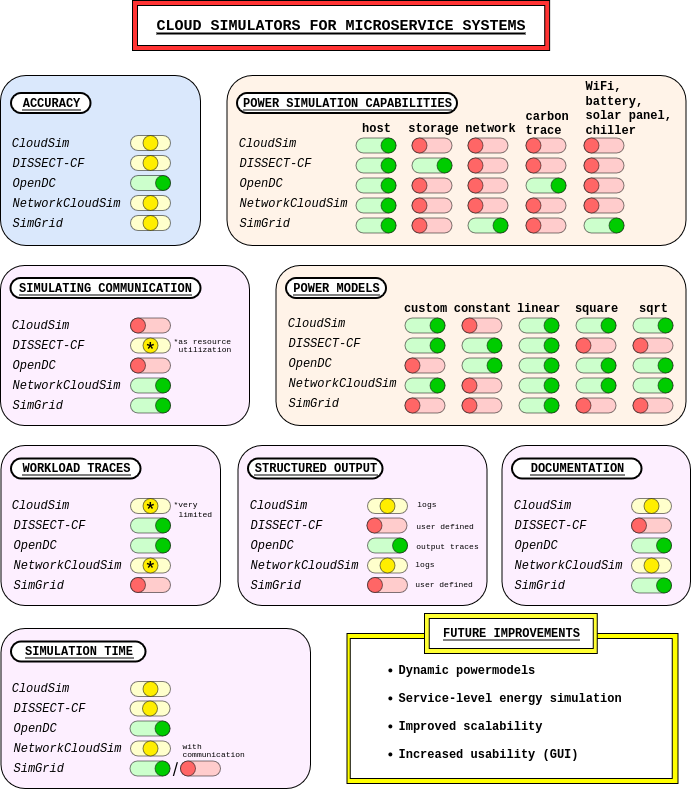
\includegraphics[width=0.85\linewidth]{figures/final.png}
    \caption{Graphic giving an overview of the discussed simulators' properties.}
    % \Description{Graphic giving an overview of the discussed simulators' properties.}
    \label{fig:final}
\end{figure*}